\chapter{Metodologia}
\label{chap:Metodo}

Neste capítulo é apresentada a metodologia de pesquisa empregada neste trabalho. Inclui os procedimentos adotados para a revisão bibliográfica, a definição do escopo, o desenvolvimento do jogo. A seguir é apresentado um diagrama na Figura \ref{Fig:all_process.png}, dando destaque às grandes fases do processo de desenvolvimento do projeto.

\begin{figure}[htbp]
	\centering
		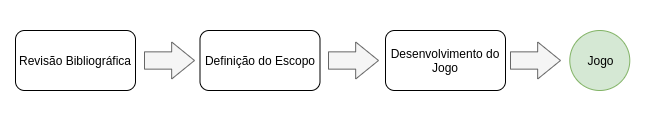
\includegraphics[keepaspectratio=true,scale=0.65]{figuras/all_process.png}
	\caption{Visão Geral do Processo Metodológico - Fonte: Mateus Augusto}
	\label{Fig:all_process.png}
\end{figure}

{\color{textmodified}
Foram adotadas algumas diretrizes e práticas da Engenharia de Software (ES) junto ao processo de construção do jogo, buscando trazer uma maior sistemática em alguns pontos do processo \cite[p. 39]{Pressman_2000} \cite[p. 31]{Bourque_2014}. Os princípios foram da metodologia de desenvolvimento em equipe Scrum, alguns princípios do Extreme Programming (XP), a Engenharia de Requisitos, o processo de construção dos protótipos, a modelagem dos dados e requisitos, a definição da arquitetura do software, a especificação dos artefatos, o processo de implementação e qualidade do software \cite[p. 74]{Pressman_2000}. Na sequência do Capítulo estão descritos os detalhes das fases do processo de desenvolvimento e evidenciadas as práticas e diretrizes de ES utilizadas. % ES pg 39 / swebok xxxi; %ES pg 74
}

\section{Revisão Bibliográfica} 

Esta seção apresenta a primeira etapa deste trabalho, a revisão bibliográfica. Em um primeiro momento, foi realizado um estudo não sistemático dos tópicos Interação Humano-Computador, Personas e Jogos.

Esta revisão foi definida seguindo a seleção de estudos relevantes para o tema designadas pelos orientadores deste trabalho. A interpretação e análise crítica das informações apresentadas na literatura adotada foram feitas pelo próprio autor deste trabalho \cite{ROTHER2007}. O Capítulo \ref{chap:ref} apresenta o resultado dessa revisão bem como uma descrição de alguns trabalhos relacionados com o tema. 

Já na busca por trabalhos correlatos foi adotada uma Revisão Sistemática de Literatura (RSL) juntamente com a técnicas de Snowballing Reveso. Detalhes sobre a metodologia usada nesta pesquisa e dos resultados obtidos estão descritos no artigo de \citeonline{deSales_SousaeSilva_2020}.

Segundo \citeonline[p. 127]{Pressman_2000} a etapa de pesquisa, revisão da literatura e análise de trabalhos semelhantes é denominada de concepção do projeto. Neste ponto são definidos o entendimento básico do problema, as partes envolvidas e demais elementos que os caracterizam. A partir da base de conhecimento formada o projeto prosseguiu para a definição do escopo, descrita na sequência.

\section{Definição do Escopo}

Essa fase tem como objetivo definir o público-alvo do jogo e identificar os requisitos que atendam aos objetivos destes jogadores. A elaboração e execução da coleta de dados utilizou-se de princípios de uma metodologia de pesquisa chamada \textit{Survey}. 

De acordo com \citeonline{Kasunic_2005} um \textit{Survey} envolve a coleta e análise de dados na qual os entrevistados respondem a um instrumento de pesquisa previamente planejado. O \textit{Survey} consiste na execução de sete principais atividades:

\begin{enumerate}
    \item Identificar os objetivos da pesquisa;
    \item Identificar e caracterizar o público-alvo;
    \item Elaborar o plano de amostragem;
    \item Elaborar e escrever o questionário;
    \item Aplicar teste piloto do questionário;
    \item Distribuir o questionário; e
    \item Analisar os resultados e escrever um relatório.
\end{enumerate}

A coleta dos dados, realizada por meio de questionário de pesquisa tem o objetivo de identificar as características dos público-alvo e realizar o levantamento de requisitos \cite[p. 128]{Pressman_2000}. A partir destes dados são definidas personas para o projeto, pois de acordo com o processo descrito em \citeauthor{usability2020} a etapa que antecede a construção das personas é a coleta de dados sobre o público-alvo. \citeonline[p. 97, 98]{cooper07} define esse processo pelas seguintes etapas:

\begin{enumerate}
    \item Identificar as variáveis comportamentais;
    \item Mapear os sujeitos da entrevista com as variáveis comportamentais;
    \item Identificar padrões de comportamento significativos;
    \item Sintetizar características e objetivos relevantes;
    \item Verificar se há redundância e integridade;
    \item Expandir a descrição de atributos e comportamentos; e
    \item Designar tipos de persona.
\end{enumerate}

Um vez definidas, as personas podem ser utilizadas em várias fases do processo. Elas servem tanto para o alinhamento de informações entre as partes envolvidas, quanto para concepção de ideias, validação dentro do projeto e tomada de decisão \cite[p. 80]{Vianna_2014}. %design things pg 80

\section{Processo de Desenvolvimento do Jogo}
\label{sec:pdj}
A partir dos dados obtidos na revisão bibliográfica e no questionário de pesquisa do \textit{Survey}, inicia-se o processo de desenvolvimento do jogo. Os requisitos, metas de experiência e o perfil do jogador identificados na fase anterior servem de base para essa etapa. Na Figura \ref{Fig:overview-process.png} é apresentada essa relação dos insumos gerados nas etapas anteriores ao processo de desenvolvimento do jogo.

\begin{figure}[htbp]
	\centering
		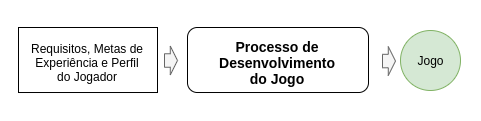
\includegraphics[keepaspectratio=true,scale=0.65]{figuras/overview-process.png}
	\caption{\textcolor{textmodified}{Relação entre Insumos e Processo de Desenvolvimento do Jogo - Fonte: Mateus Augusto}}
	\label{Fig:overview-process.png}
\end{figure}

Neste trabalho, o \textit{Playcentric Design Process} \cite{Fullerton_2008}, um método usado para desenvolvimento de jogos digitais, foi adotado como o cerne da fase de desenvolvimento do PersonaDesignGame. Mais detalhes sobre o \textit{Playcentric Design Process} (PDP) podem ser vistos no próximo Capítulo, na Seção \ref{sec:play}.

Este método se baseia em um princípio iterativo na construção do jogo e interativo com os jogadores-alvo. Para isso, neste trabalho faz-se uso das personas, sendo que estas são diretamente relacionadas as metas de experiência e perfil dos jogadores-alvo, que são o ponto de partida para inicio do desenvolvimento do jogo, de acordo com o PDP \citeonline[p. 10, 11]{Fullerton_2008}.

Tendo em vista o princípio deste método, o desenvolvimento do PersonaDesignGame (PDG) segue os sete passos definidos no \textit{Playcentric Design Process}. Complementarmente ao PDP foram utilizadas as diretrizes e práticas da Engenharia de Software. A seguir estão descritos os passos para o desenvolvimento do PDG: 

No primeiro passo é iniciada a tarefa de modelagem dos requisitos elicitados, onde as informações obtidas no levantamento de requisitos são refinadas e cujo nível de abstração já demonstra o comportamento do software \cite[p. 128]{Pressman_2000}. Os produtos deste passo já são todos formalizados e já documentados em artefatos iniciais.
   
O segundo passo conta com a elaboração de um protótipo de papel \cite[p. 262, 263]{Preece_Rogers_Sharp_2005}. Este simula as interações principais do jogo, tendo em vista elaborar e fazer alterações no design do jogo, interagindo com o jogador e as personas, testando e validando os conceitos iniciais levantados \cite[p. 15]{Fullerton_2008}. Já neste passo é buscado evidenciar a percepção dos jogadores e das personas quanto às metas de experiência definidas. Os resultados deste processo são também formalizados e documentados.

Este terceiro passo é opcional no \textit{Playcentric Design Process}, porém para este trabalho acaba sendo obrigatório e realizado em três momentos, TCC 1.1, TCC1.2 e TCC 2 como é apresentado na Seção \ref{sec:plano_trab}, no Capítulo \ref{chap:intro}. As apresentações são marcos para o projeto, onde é demonstrado às partes interessadas, uma banca examinadora, o desenvolvimento do jogo e no caso, a defesa do TCC. Assim é possível receber um \textit{feedback} da banca sobre o jogo proposto e a partir disso realizar alterações e melhorias, que são refletidas nos documentos e artefatos iniciais do projeto \cite[p. 15]{Fullerton_2008}. 

Em seguida o quarto passo é realizado a partir do protótipo de papel e demais artefatos elaborado. Assim é criado o protótipo de alta-fidelidade. Focado ainda na validação de conceitos e não na produção do jogo este passo visa a praticidade. Seguindo o fluxo iterativo, o protótipo elaborado representa apenas interações relevantes, e assim é testado pelos jogadores e pelas personas. Caso demonstre uma jogabilidade funcional que atinja as metas de experiência do jogador o processo segue para o próximo passo \cite[p. 15]{Fullerton_2008}. A documentação e demais artefatos do projeto são então atualizados. 

Neste ponto, o quinto passo, são especificadas todas as ideias concebidas, prototipadas, testadas, validadas e já brevemente documentadas nos passos anteriores \cite[p. 15]{Fullerton_2008}. Assim é elaborado o \textit{Game Design Document} (GDD), contendo as características relevantes para o jogo, como a mecânica, fluxo, regras e entre outros elementos \cite[p. 101]{Bethke_2003}. Outro documento que auxilia na especificação do projeto, no caso de um jogo digital, é o \textit{Technical Design Document} (TDD), que trata não apenas do que precisa ser criado, mas também como será implementado, contemplando a arquitetura do software, modelagem de dados, requisitos e entre outros aspectos técnicos \cite[p. 129]{Bethke_2003}.

No sexto passo é criada a arte final para o jogo, reaproveitando ao máximo o que foi produzido no protótipo de alta-fidelidade, e também é desenvolvido o código do software do jogo \cite[p. 15, 18]{Fullerton_2008}. A metodologia de desenvolvimento adotada se baseia nas diretrizes do Scrum \cite{schwaber2002agile}, XP \cite{lindstrom2004extreme} e Kanban \cite{kniberg2010kanban}. Mesmo neste passo mais avançado podem haver mudanças, sendo assim, caso ocorram, ajustes são feito seguindo o mesmo princípio iterativo aplicado nos passos anteriores e seguindo com as mudanças necessárias na documentação. 
    
Por fim, neste último passo, o sétimo, o jogo é testado e avaliado pelos jogadores e personas, evidenciando se tal atende às expectativas de experiência de jogo esperadas \cite[p. 18]{Fullerton_2008}. % Playcentric pg 18

Finalizado o capítulo sobre a metodologia, é apresentado no capítulo seguinte o referencial teórico. Esta parte do trabalho já é reflexo do resultado da primeira etapa do processo metodológico, que contempla a revisão da literatura.

% Trazer uma sessão falando das práticas ágeis adotadas?

% TCC 2
%   - Pesquisa Científica:
%      - Apresentação dos Resultados
%      - Considerações Finais e Sugestão de Trabalhos Futuros
%   - Desenvolvimento de Software
%      - Gerência e Configuração do Ambiente (qualidade de escrita de código, bibliotecas, dependências, ferramentas, testes)
%      - Implementação 
%      - Testes 
%   - Continuidade do Projeto
%    - Elaborar Artefatos
%      - Artefatos de Design
%      - Artefatos Técnicos
